\chapter{Arhitektura i dizajn sustava}

		\noindent\textit{Arhitektura se može podijeliti na 3 djela: }
		\begin{packed_item}
			\item \textbf{Korisničko sučelje(frontend)} Predstavlja sve što korisnik vidi. Prikazuje korisničko sučelje, prenosi podatke od korisnika na backend i obrnuto.
			\item \textbf{Aplikacijski sloj(backend)}
			Bavi se procesiranje podataka koje korisnik zatraži preko frontenda. Obrađuje i validira podatke, te pohranjuje i dohvaća podatke iz baze.
			\item \textbf{Baza podataka}
			U bazu podataka se spremaju svi podatci. Služi za lakše spremanje, dohvaćanje i održavanje integriteta podadtaka.
		\end{packed_item}
		
	
		
		\noindent Backend dio aplikacije je rađen u javi korištenjem spring boot alata. Dok je frontend rađen u react-u, proramskim jezikom javascript. Za razvojno okruženje frontenda korišten je Microsoft visual studio, a za backend IntelliJ IDEA. Arhitektura susava temeljena je na MVC(Model-View-Controller) modelu. Prednost takve arhitekture je što su komponente neovisne te mogu biti testirane zasebno što olakšava proširivanje, testiranje i održavanje aplikacije.
		
		\begin{packed_item}
	\item \textbf{Model} Predstavlja poslovnu logiku i podatke aplikacije. Ovdje se definiraju objekti i logika koji se koriste za dohvaćanje, ažuriranje i pohranu podataka. Ne ovisi o korisničkom sučelju.
	\item \textbf{View)}
	Predstavlja korisničko sučelje i odgovoran je za prikaz podataka. Ne sadrži poslovnu logiku i ne komunicira izravno s Modelom. Ažurira se na temelju promjena u Modelu.
	\item \textbf{Controller}
	Obradjuje korisničke zahtjeve i ažurira Model te odabire pravi View za prikaz. Glavna uloga je upravljati komunikacijom između Modela i Viewa. Ovisno o korisničkom zahtjevu, Controller može ažurirati Model, ažurirati View ili oboje.
\end{packed_item}
		

				
		\section{Baza podataka}
	Baza podataka služi nam za jednostavniju i bržu pohranu i dohvat podataka. Za našu aplikaciju koristili smo relacijsku bazu podataka. Osnovna struktura baze su povezane tablice koje su određene imenom i skupom atributa. Baza podataka sastoji se od sljedećih tablica: 
		
		\begin{packed_item}
			\item {Users}
			\item {Children}
			\item {ChildRegister}
			\item {ChildExaminations}
			\item {MedicalCertificates}
			\item {TestResults}
			\item {Notifications}
			\item {SpecialistAppointments}
			\item {VisitHistory}
		\end{packed_item}
		
			\subsection{Opis tablica}
			

		\noindent \textbf{User} entitet sastoji se od atributa: ID, userName, password, firstName, lastName, email, role. Entitet sadrži sve atribute vezane za korisnike koji su nam potrebni u izradi aplikacije. Ovaj entitet je u vezi Many-to-Many s entitetom Children preko ID atributa korisnika, One-to-Many vezom s entitetom Notifications preko atributa ID korisnik, One-to-Many vezom s entitetom SpecialistAppointments preko atributa ID korisnika, One-to-Many vezom s entitetom VisitHistory preko atributa ID korisnika i One-to-Many vezom s entitetom ChildExaminations preko atributa ID korisnika.
				
				
				\begin{longtblr}[
					label=none,
					entry=none
					]{
						width = \textwidth,
						colspec={|X[6,l]|X[6, l]|X[20, l]|}, 
						rowhead = 1,
					} %definicija širine tablice, širine stupaca, poravnanje i broja redaka naslova tablice
					\hline \SetCell[c=3]{c}{\textbf{Users}}	 \\ \hline[3pt]
					\SetCell{LightGreen}ID & INT	&  	Jedinstven identifikator korisnika 	\\ \hline
					userName	& VARCHAR & jedinstven naziv korisnika   	\\ \hline 
					password & VARCHAR & lozinka  \\ \hline 
					firstName & VARCHAR	& ime korisnika 		\\ \hline 
					lastName	& VARCHAR & prezime korisnika  	\\ \hline 
					email & VARCHAR & e-mail adresa korisnika \\ \hline
					role & VARCHAR & uloga korisnika \\ \hline
				\end{longtblr}
				
			\noindent \textbf{Children} entitet sastoji se od atributa: ID, name, dateOfBirth, oib i parentID. Entitet sadrži sve atribute vezane za djecu koji su nam potrebni u izradi aplikacije. Ovaj entitet je u vezi Many-to-Many s entitetom User preko parentID atributa, Many-to-One vezom s entitetom ChildRegister preko atributa ID djeteta, One-to-Many vezom s entitetom ChildExaminations preko atributa oib, One-to-Many vezom s entitetom MedicalCertificates preko atributa oib, One-to-Many s entitetom TestResults preko atributa oib te One-to-Many vezom s entitetom SpecialistAppointments preko atributa ID.
				
				\begin{longtblr}[
					label=none,
					entry=none
					]{
						width = \textwidth,
						colspec={|X[6,l]|X[6, l]|X[20, l]|}, 
						rowhead = 1,
					} %definicija širine tablice, širine stupaca, poravnanje i broja redaka naslova tablice
					\hline \SetCell[c=3]{c}{\textbf{Children}}	 \\ \hline[3pt]
					\SetCell{LightGreen}ID & INT	&  	Jedinstven identifikator djeteta	\\ \hline
					name	& VARCHAR & ime djeteta   	\\ \hline 
					dateOfBirth & DATETIME & datum rođenja djeteta  \\ \hline 
					oib & iNT	& osobni identifikacijski broj djeteta 		\\ \hline 
					\SetCell{LightBlue} parentID	& INT & jedinstven identifikator roditelja  	\\ \hline 
				\end{longtblr}
				
				\noindent \textbf{ChildRegisters} entitet sastoji se od atributa: ID, childID i basicInfo. Entitet sadrži sve atribute za registar djece koji su nam potrebni u izradi aplikacije. Ovaj entitet je u vezi One-to-Many s entitetom Children preko ID atributa.
				
				\begin{longtblr}[
					label=none,
					entry=none
					]{
						width = \textwidth,
						colspec={|X[6,l]|X[6, l]|X[20, l]|}, 
						rowhead = 1,
					} %definicija širine tablice, širine stupaca, poravnanje i broja redaka naslova tablice
					\hline \SetCell[c=3]{c}{\textbf{ChildRegisters}}	 \\ \hline[3pt]
					\SetCell{LightGreen}ID & INT	&  	Jedinstven identifikator registra	\\ \hline
					\SetCell{LightBlue}ChildID	& INT & jedinstven identifikator djeteta   	\\ \hline 
					basicInfo & VARCHAR & osnovni podatci djeteta  \\ \hline 
				\end{longtblr}
				
				\noindent \textbf{ChildExaminations} entitet sastoji se od atributa: ID, oibChild, pediatritionID, dateOfExam, diagnosis, sickLeave. Entitet sadrži sve atribute za pregled djece koji su nam potrebni u izradi aplikacije. Ovaj entitet je u vezi Many-to-One s entitetom Children preko oibChild atributa, Many-to-One vezom s entitetom User preko atributa pediatritionID.
							
				\begin{longtblr}[
					label=none,
					entry=none
					]{
						width = \textwidth,
						colspec={|X[6,l]|X[6, l]|X[20, l]|}, 
						rowhead = 1,
					} %definicija širine tablice, širine stupaca, poravnanje i broja redaka naslova tablice
					\hline \SetCell[c=3]{c}{\textbf{ChildExaminations}}	 \\ \hline[3pt]
					\SetCell{LightGreen}ID & INT	&  	jedinstven identifikator pregleda	\\ \hline
					\SetCell{LightBlue}oibChild	& INT & jedinstven identifikator djeteta   	\\ \hline 
					\SetCell{LightBlue}pediatritionID & INT & jedinstven identifikator pedijatra \\ \hline 
					dateOfExam & DATETIME	& datum pregleda 		\\ \hline 
					diagnosis	& VARCHAR & dijagnoza djeteta 	\\ \hline 
					sickLeave & VARCHAR & preporuka za bolovanje \\ \hline
				\end{longtblr}
				
			\noindent \textbf{MedicalCertificates} entitet sastoji se od atributa: ID, oibChild, dateOfCert, reason, pedConf. Entitet sadrži sve atribute za ispričnice koji su nam potrebni u izradi aplikacije. Ovaj entitet je u vezi Many-to-One s entitetom Children preko oibChild atributa.
				
				\begin{longtblr}[
					label=none,
					entry=none
					]{
						width = \textwidth,
						colspec={|X[6,l]|X[6, l]|X[20, l]|}, 
						rowhead = 1,
					} %definicija širine tablice, širine stupaca, poravnanje i broja redaka naslova tablice
					\hline \SetCell[c=3]{c}{\textbf{MedicalCertificates}}	 \\ \hline[3pt]
					\SetCell{LightGreen}ID & INT	&  	Jedinstven identifikator ispričnice	\\ \hline
					\SetCell{LightBlue}oibChild	& INT & osobni identifikacijski broj djeteta   	\\ \hline 
					dateOfCert & DATETIME & datum izdavanja ispričnice  \\ \hline 
					reason & VARCHAR	& razlog izdavanja ispričnice	\\ \hline 
					pedConf	& VARCHAR & potvrda pedijatra  	\\ \hline 
				\end{longtblr}
				
				\noindent \textbf{TestResults} entitet sastoji se od atributa: ID, oibChild, dateOfTest, typeOfResult i result. Entitet sadrži sve atribute za nalaze koji su nam potrebni u izradi aplikacije. Ovaj entitet je u vezi Many-to-One s entitetom Children preko oibChild atributa.
				
				\begin{longtblr}[
					label=none,
					entry=none
					]{
						width = \textwidth,
						colspec={|X[6,l]|X[6, l]|X[20, l]|}, 
						rowhead = 1,
					} %definicija širine tablice, širine stupaca, poravnanje i broja redaka naslova tablice
					\hline \SetCell[c=3]{c}{\textbf{TestResults}}	 \\ \hline[3pt]
					\SetCell{LightGreen}ID & INT	&  	Jedinstven identifikator nalaza	\\ \hline
					\SetCell{LightBlue}oibChild	& INT & osobni identifikacijski broj djeteta   	\\ \hline 
					dateOfTest & DATETIME & datum izdavanja nalaza  \\ \hline 
					typeOfResult & VARCHAR	& vrsta nalaza	\\ \hline 
					result	& VARCHAR & rezultati nalaza  	\\ \hline 
				\end{longtblr}
				
				\noindent \textbf{Notifications} entitet sastoji se od atributa: ID, textOfNotif, dateOfNotif i receiverID. Entitet sadrži sve atribute za obavijesti koji su nam potrebni u izradi aplikacije. Ovaj entitet je u vezi Many-to-One s entitetom User preko receiverID atributa.
				
				\begin{longtblr}[
					label=none,
					entry=none
					]{
						width = \textwidth,
						colspec={|X[6,l]|X[6, l]|X[20, l]|}, 
						rowhead = 1,
					} %definicija širine tablice, širine stupaca, poravnanje i broja redaka naslova tablice
					\hline \SetCell[c=3]{c}{\textbf{Notifications}}	 \\ \hline[3pt]
					\SetCell{LightGreen}ID & INT	&  	Jedinstven identifikator obavijesti	\\ \hline
					textOfNotif & VARCHAR & datum izdavanja ispričnice  \\ \hline 
					dateOfNotif & DATETIME	& datum slanja obavijesti\\ \hline 
					\SetCell{LightBlue}receiverID	& INT & identifikator primatelja obavijesti   	\\ \hline 
				\end{longtblr}
				
				\noindent \textbf{SpecialistAppointments} entitet sastoji se od atributa: ID, patientID, dateOfApp, location, conformation. Entitet sadrži sve atribute za specijalne preglede koji su nam potrebni u izradi aplikacije. Ovaj entitet je u vezi Many-to-One s entitetom Children preko patientID atributa i Many-to-One vezom s entitetom user preko patientID atributa.
				
				\begin{longtblr}[
					label=none,
					entry=none
					]{
						width = \textwidth,
						colspec={|X[6,l]|X[6, l]|X[20, l]|}, 
						rowhead = 1,
					} %definicija širine tablice, širine stupaca, poravnanje i broja redaka naslova tablice
					\hline \SetCell[c=3]{c}{\textbf{SpecialistAppointments}}	 \\ \hline[3pt]
					\SetCell{LightGreen}ID & INT	&  	Jedinstven identifikator pregleda	\\ \hline
					\SetCell{LightBlue}patientID	& INT & jedinstveni identifikator pacijenta   	\\ \hline 
					dateOfApp & DATETIME & datum pregleda \\ \hline 
					location & VARCHAR	& lokacija pregleda	\\ \hline 
					conformation & VARCHAR & potvrda liječnika o naručivanju  	\\ \hline 
				\end{longtblr}
				
				\noindent \textbf{VisitHistory} entitet sastoji se od atributa: ID, userID, dateOfVisit i diagnosis. Entitet sadrži sve atribute za povijest posjeta koji su nam potrebni u izradi aplikacije. Ovaj entitet je u vezi Many-to-One s entitetom user preko userID atributa.
				
				\begin{longtblr}[
					label=none,
					entry=none
					]{
						width = \textwidth,
						colspec={|X[6,l]|X[6, l]|X[20, l]|}, 
						rowhead = 1,
					} %definicija širine tablice, širine stupaca, poravnanje i broja redaka naslova tablice
					\hline \SetCell[c=3]{c}{\textbf{VisitHistory}}	 \\ \hline[3pt]
					\SetCell{LightGreen}ID & INT	&  	Jedinstven identifikator posjeta	\\ \hline
					\SetCell{LightBlue}userID	& INT & jedinstveni identifikator pacijenta  	\\ \hline 
					dateOfVisit & DATETIME & datum posjeta  \\ \hline 
					diagnosis & VARCHAR	& dijagnoza	\\ \hline 
				\end{longtblr}
				
			
			\subsection{Dijagram baze podataka}
				\includegraphics[scale=0.6]{dijagrami/Bazapodataka.PNG}
			
			\eject
			
			
		\section{Dijagram razreda}
		\begin{figure}[H]
			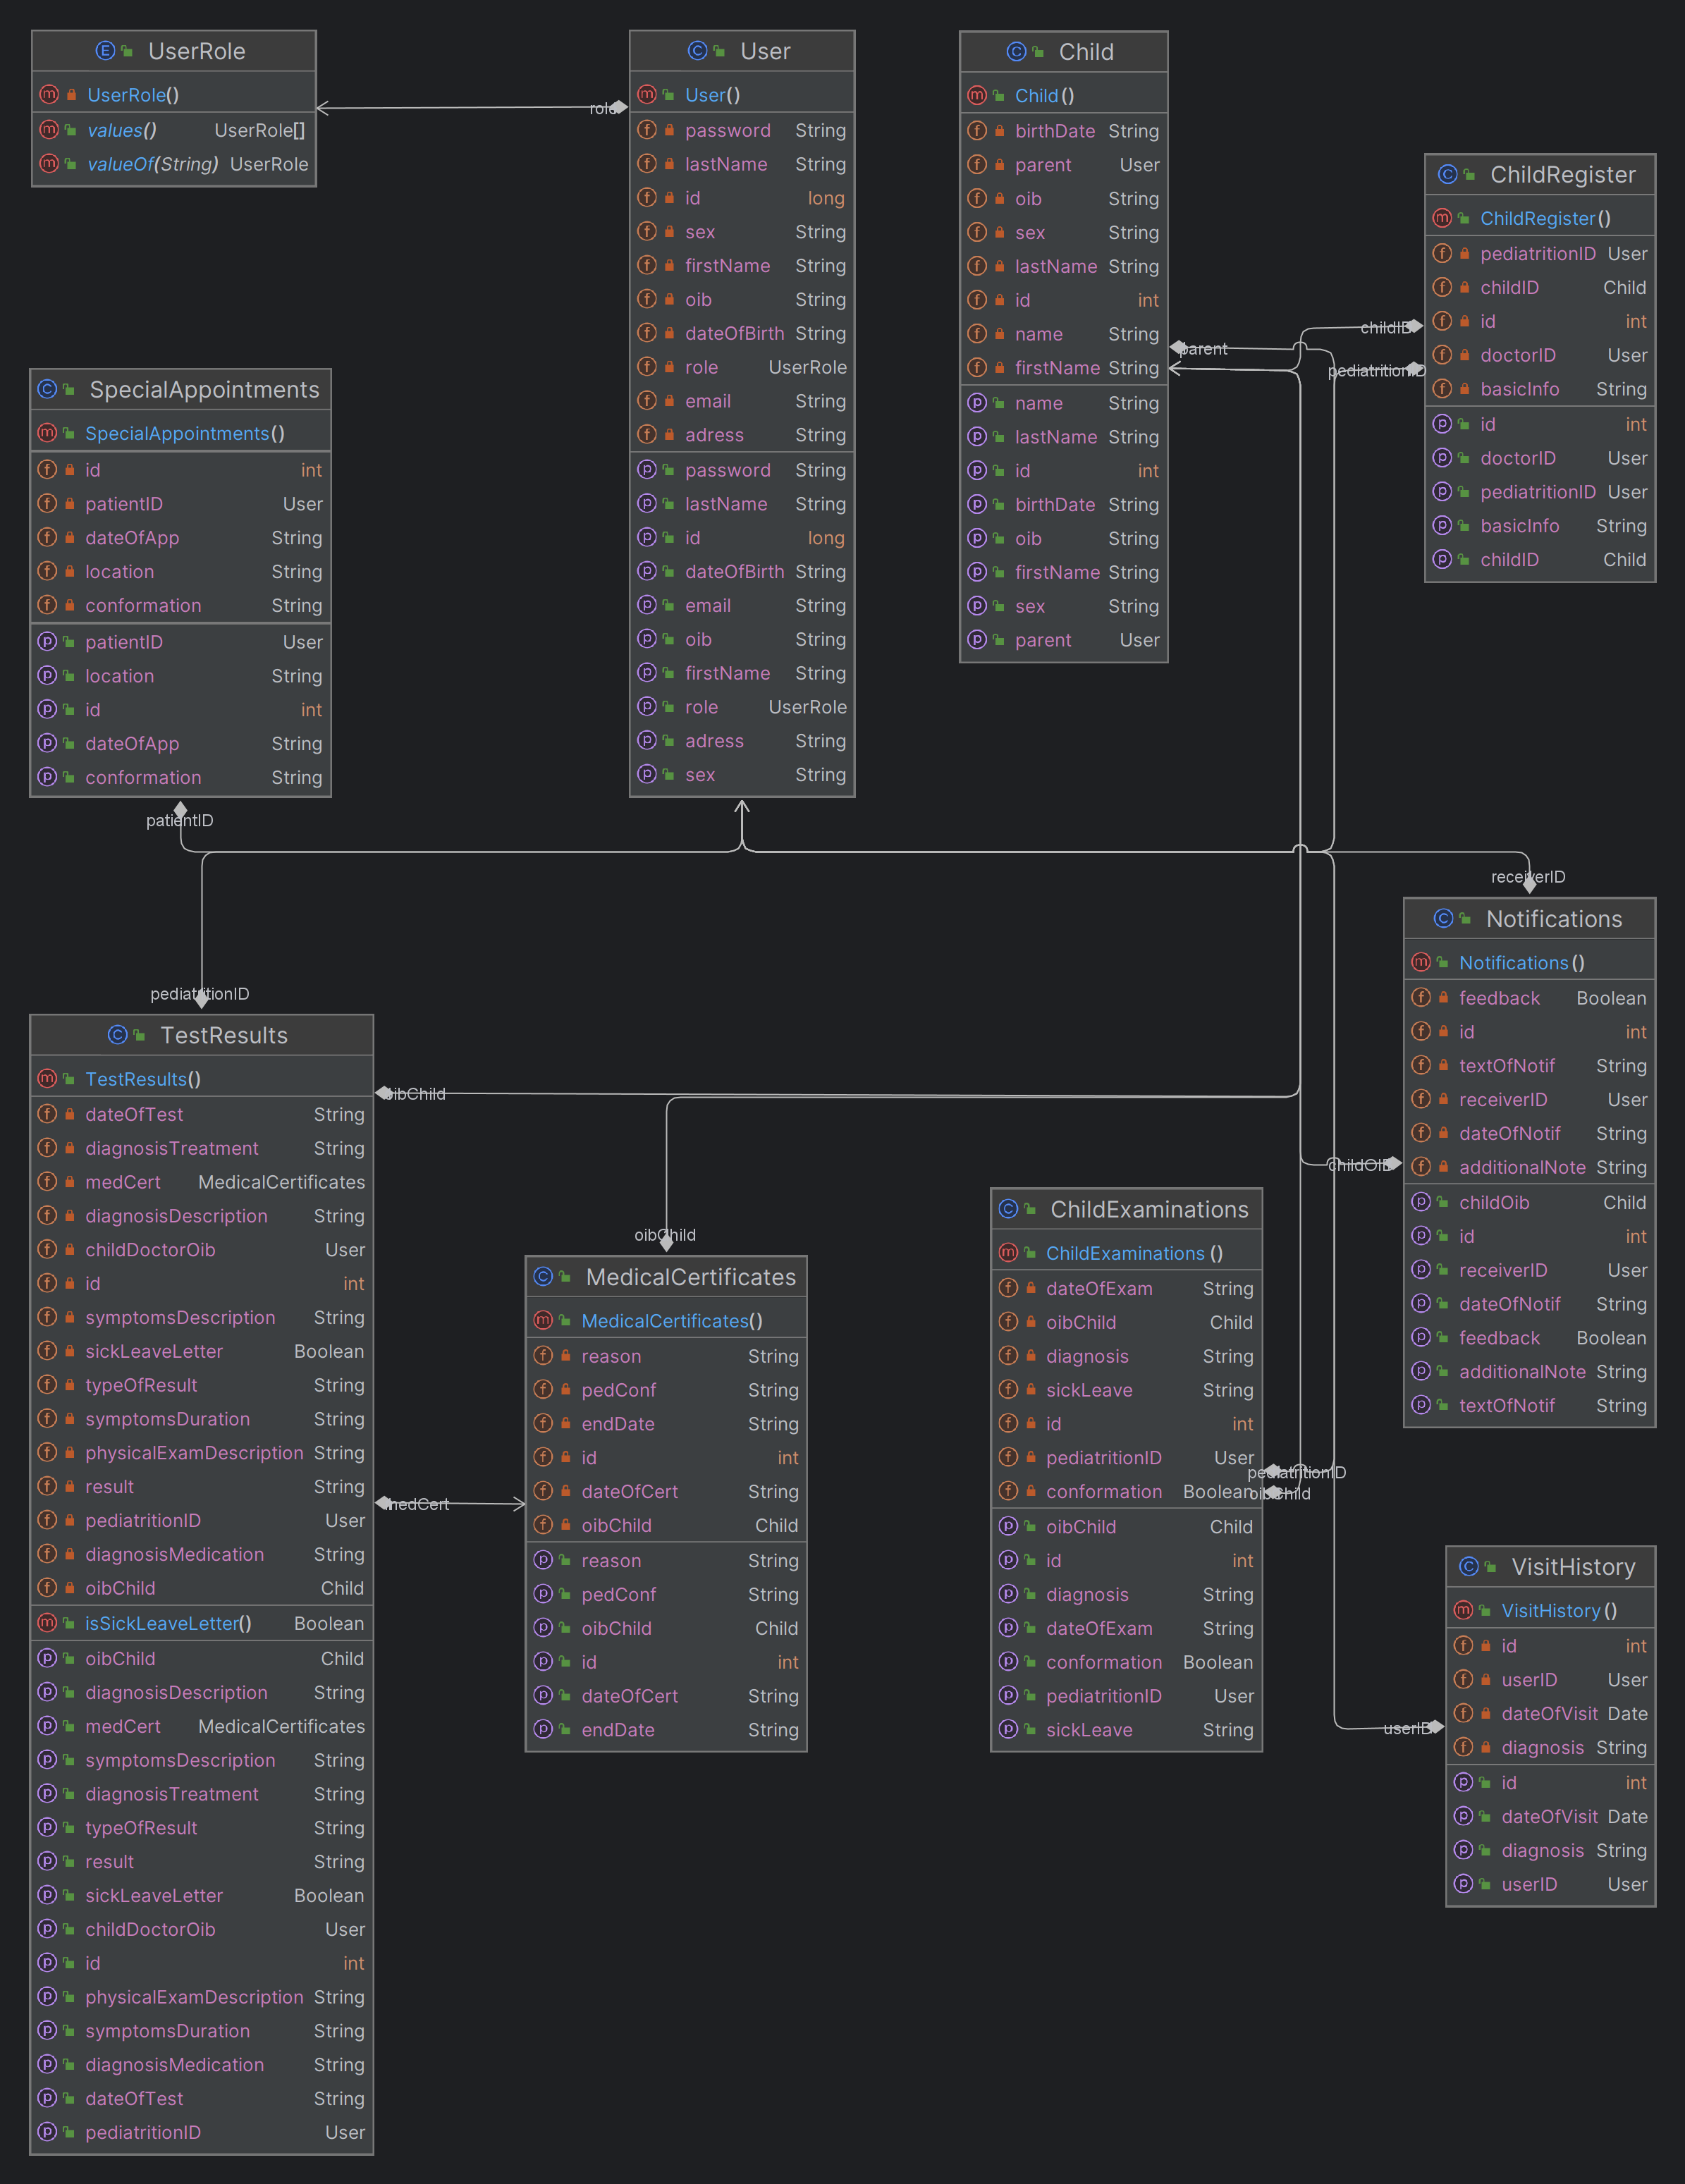
\includegraphics[width=15cm, height=12cm]{dijagrami/class_diagram.png}
			\caption{Dijagram razreda}
			\label{fig:classD}
		\end{figure}
		\eject
		
		\section{Dijagram stanja}
			
			
			\begin{figure}[H]
				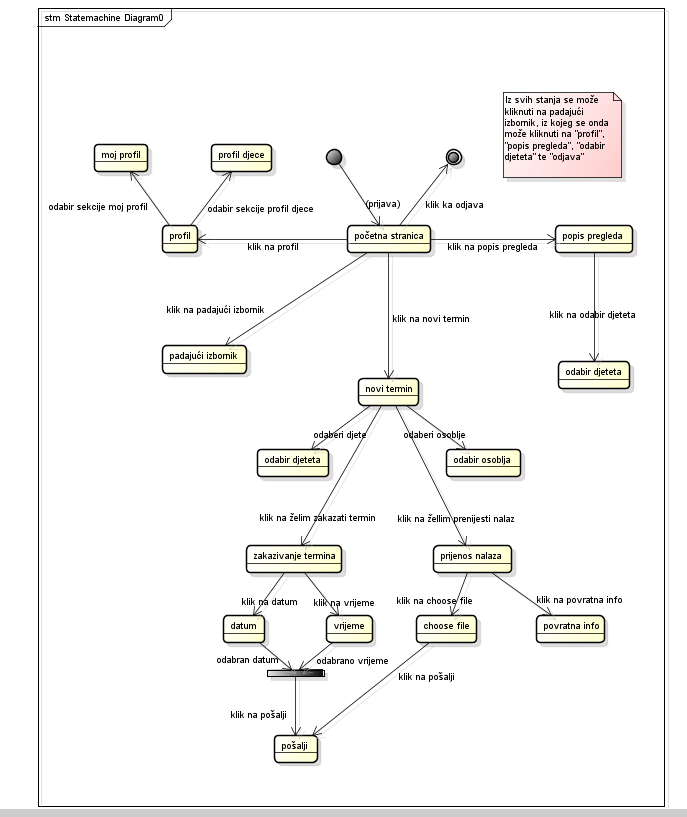
\includegraphics[]{dijagrami/dijagram_stanja.png}
				\caption{Dijagram stanja}
				\label{fig:dijagramStanja}
			\end{figure}
			
			Na priloženom dijagramu stanja prikazano je stanje za prijavljenog korisnika. Nakon prijave korisniku se prikazuje naslovna stranica. Sa naslovne stranice pomoću padajućeg izbornika korisnik može dogovoriti novi termin, pregledati vlastiti profil i popis pregleda te odjaviti se. Klikom na profil prikazuju mu se njegovi podatci ili podatci njegove djece. Klikom na novi termin korisnik može dogovoriti novi termin ili prenijeti dokument u kojem se nalazi njegov nalaz. U svakom trenutku korisnik se preko padajućeg izbornika može vratiti na naslovnu stranicu, odjaviti se te izabrati "profil", "popis pregleda" ili "novi termin".
			
			
			\eject 
		
		\section{Dijagram aktivnosti}
			
			\begin{figure}[H]
				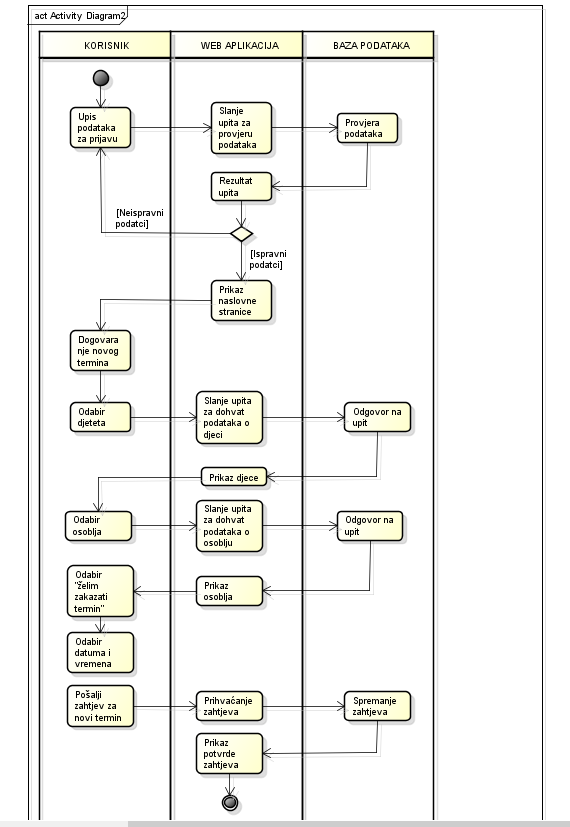
\includegraphics[scale=1.1]{dijagrami/dijagram_aktivnosti.png}
				\centering
				\caption{Dijagram aktivnosti}
				\label{fig:dijagramAktivnosti}
			\end{figure}
			
			Priloženi dijagram aktivnosti prikazuje proces naručivanja na novi termin. Korisnik se prvo prijavi u sustav. Zatim za novi termin odabere djete i osoblje te ispuni datum i vrijeme. Kada je sve od navedenog odabrao te ispunio, korisnik pošalje svoj zahtjev čime on postaje aktivan u sustavu.
			
			\eject
		\section{Dijagram komponenti}
		
			\textbf{\textit{dio 2. revizije}}\\
		
			 \textit{Potrebno je priložiti dijagram komponenti s pripadajućim opisom. Dijagram komponenti treba prikazivati strukturu cijele aplikacije.}
